\DailyTitle{6275 Log (October 8, 2010)}

\DailySection{Goals}

\begin{enumerate}
\item Make a list of things that need to be documented for the ZJet candle analysis
\item Check what Artur needs in terms of vecbos ntuples.  Check out new ntuple dumper code and test run.
\item Try out Hcal DQM test bench on lxplus.
\item Double-spike algorithm.
\end{enumerate}

\DailySection{Summary List}

\begin{enumerate}
\item Yay
\end{enumerate}

\DailySection{Checking out new vecbos ntuple producer code}

Followed the instruction in \url{http://cmssw.cvs.cern.ch/cgi-bin/cmssw.cgi/UserCode/HiggsAnalysis/HiggsToWW2e/doc/README?revision=1.57},
except that the version is changed to \texttt{CMSSW} \texttt{3\_8\_2}.

\begin{verbatim}
scramv1 project CMSSW CMSSW_3_9_0_pre1
cd CMSSW_3_9_0_pre1/src
eval `scramv1 runtime -sh`

cvs co -r V04-3_9_X -d HiggsAnalysis/HiggsToWW2e UserCode/HiggsAnalysis/HiggsToWW2e
cvs co -r V00-3_5_X -d Configuration/ElectronIdentification \\
   UserCode/emanuele/Configuration/ElectronIdentification
addpkg RecoEgamma/ElectronIdentification
cvs co -r V02-3_6_0 -d MyAnalysis/IsolationTools \\
   UserCode/emanuele/MyAnalysis/IsolationTools

cp /afs/cern.ch/user/e/emanuele/public/4Likelihood/PDFsSQLite/CMSSW_3_2_X/electronIdLikelihoodTkIsolated.db \\
   HiggsAnalysis/HiggsToWW2e/test/python
cd RecoEgamma/ElectronIdentification/python/
rm likelihoodPdfsDB_cfi.py
wget http://emanuele.web.cern.ch/emanuele/ElectronID/patchLikelihoodDb/likelihoodPdfsDB_cfi.py
cd -

scramv1 build
\end{verbatim}

It builds fine.

\DailySection{Hcal pulse shape fitting}

The long process from yesterday with \texttt{RooFit} finally ended after a few hours, and that's only a small percentage of the total events.
And.....it doesn't look good.  Signal distribution and noise distribution look the same.  The black box named \texttt{RooFit} is too complicated,
and it's hard to guess what really is happening.  One iteration takes hours so it's bad.

So I tried to mathematically calculate the minimum and implement the result.  Suppose $T_i$ is the ten pedestal-subtracted charges, and
$F_i$ is the pulse shape, integrated into 25ns time slices.  Then the only free parameter to fit to is $\alpha$, the overall scale.  So

\begin{eqnarray}
Error^2 &=& \sum_{i=0}^{9} (T_i - \alpha F_i)^2\nonumber\\
   &=& \sum_{i=0}^{9} T_i^2 - 2 \alpha \sum_{i=0}^{9} T_i F_i + \alpha^2 \sum_{i=0}^{9} F_i^2\nonumber\\
\dfrac{d(Error^2)}{d\alpha} &=& -2\sum_{i=0}^{9} T_i F_i + 2\alpha \sum_{i=0}^{9} F_i^2 = 0\nonumber\\
\alpha &=& \dfrac{\displaystyle\sum_{i=0}^{9} T_i F_i}{\displaystyle\sum_{i=0}^{9} F_i^2}\nonumber\\
\min (Error^2) &=& \sum_{i=0}^{9} T_i^2 - \dfrac{\left(\displaystyle\sum_{i=0}^{9} T_i F_i\right)^2}{\displaystyle\sum_{i=0}^{9} F_i^2}\nonumber
\end{eqnarray}

Now all I need to do is to scan through different possible offsets (in units of ns), calculate the above quantity, and find the minimum.
This works pretty well.  Now the whole thing finishes within a couple minutes.  And the result makes sense.
One possible upgrade is to go down to sub-ns after the minimum region is identified....but let's not worry about that now.
The fit result is shown in figures \ref{Figure_6275HHcalPulseFitError}, \ref{Figure_6275HHcalPulseFitError100},
\ref{Figure_6275HHcalPulseFitTime} and \ref{Figure_6275HHcalPulseFitTime100}.
Preliminary (just plotted) results on test statistics are shown in figures
\ref{Figure_6275HTestStatisticsLinearFit}, \ref{Figure_6275HTestStatisticsLinearFit100}, \ref{Figure_6275HTestStatisticsLinearFitVsCharge},
\ref{Figure_6275HTestStatisticsTwoLevelFit}, \ref{Figure_6275HTestStatisticsTwoLevelFit100}, \ref{Figure_6275HTestStatisticsTwoLevelFitVsCharge},
\ref{Figure_6275HTestStatisticsRMS9} and \ref{Figure_6275HTestStatisticsRMS9100}.

As a next step I should upgrade all $Error^2$ to $\chi^2$.  I don't even need the conversion factor from charge to number of photoelectron!
All that matters is the square-root dependence, and any additional factor will show up as shifts in the test variable.  Plus, the factor will cancel away
when I take the ratio....  This is for the weekend\tweakedtilde

\begin{figure}
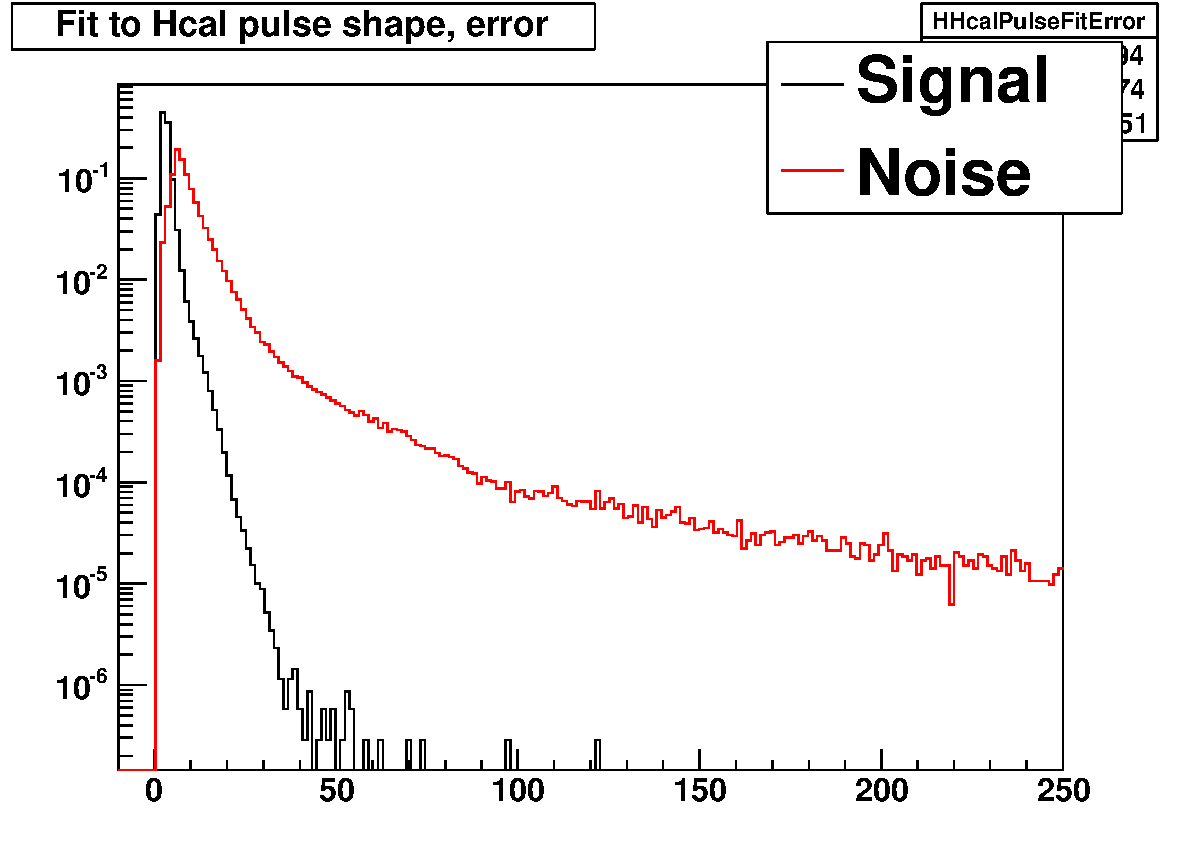
\includegraphics[width=120mm]{DailyLog/6275/6275HHcalPulseFitError.pdf}
\caption{Error from fit to nominal shape using the above custom method.}
\label{Figure_6275HHcalPulseFitError}
\end{figure}

\begin{figure}
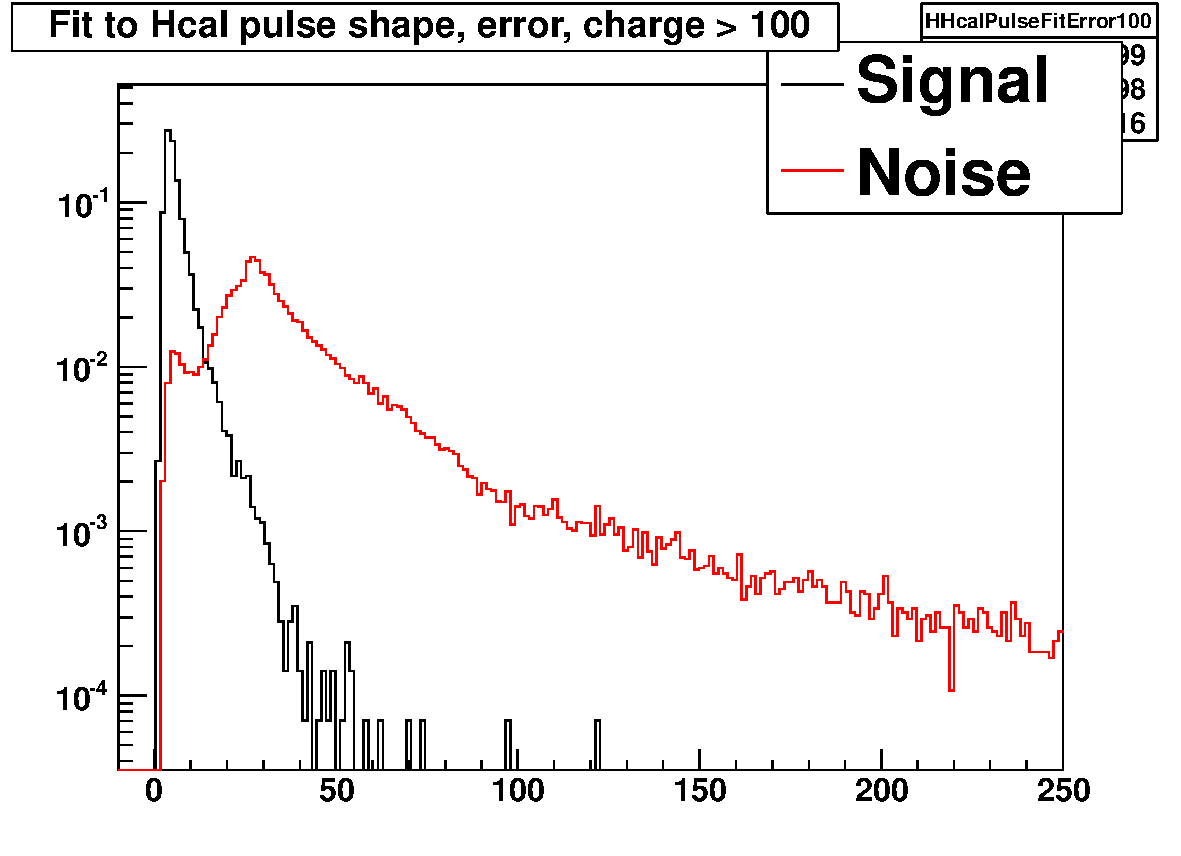
\includegraphics[width=120mm]{DailyLog/6275/6275HHcalPulseFitError100.pdf}
\caption{Error from fit for pulse with charge at least 100 fC}
\label{Figure_6275HHcalPulseFitError100}
\end{figure}

\begin{figure}
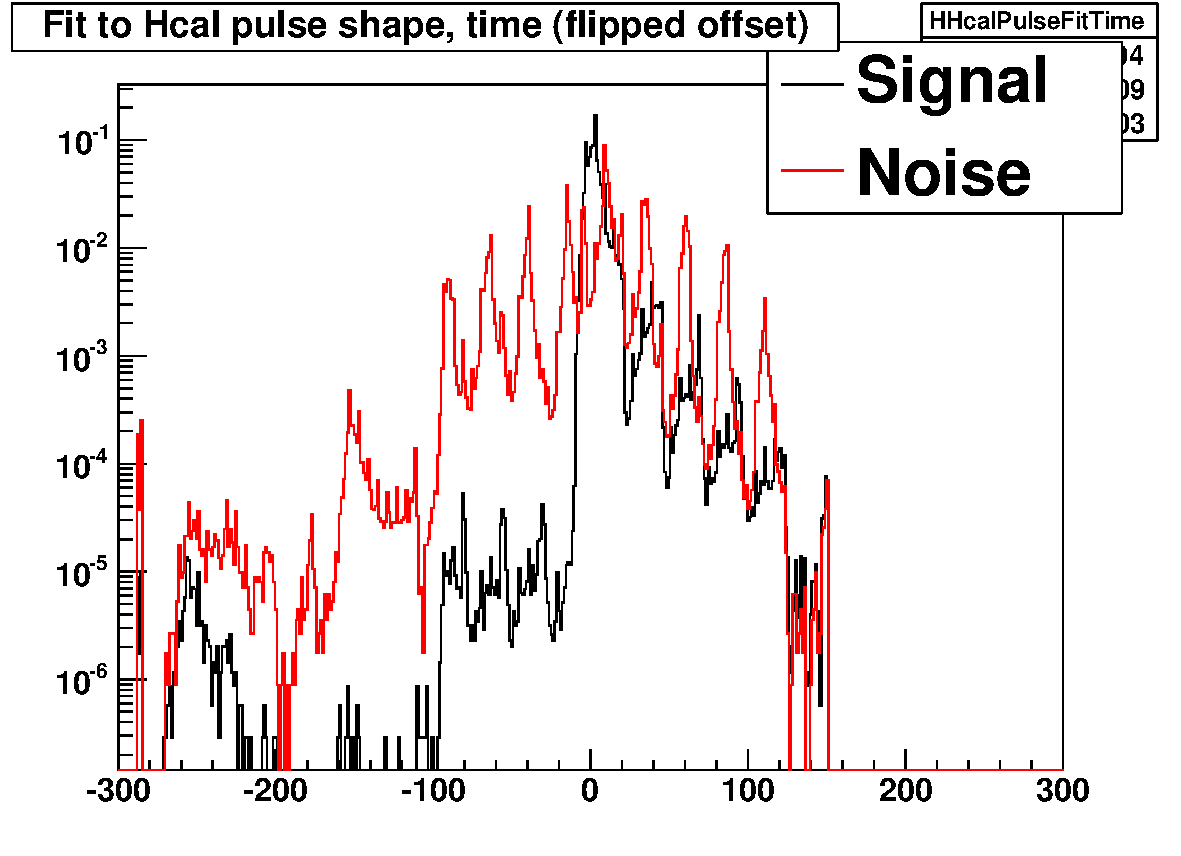
\includegraphics[width=120mm]{DailyLog/6275/6275HHcalPulseFitTime.pdf}
\caption{Peak time from fit to nominal shape using the above custom method.}
\label{Figure_6275HHcalPulseFitTime}
\end{figure}

\begin{figure}
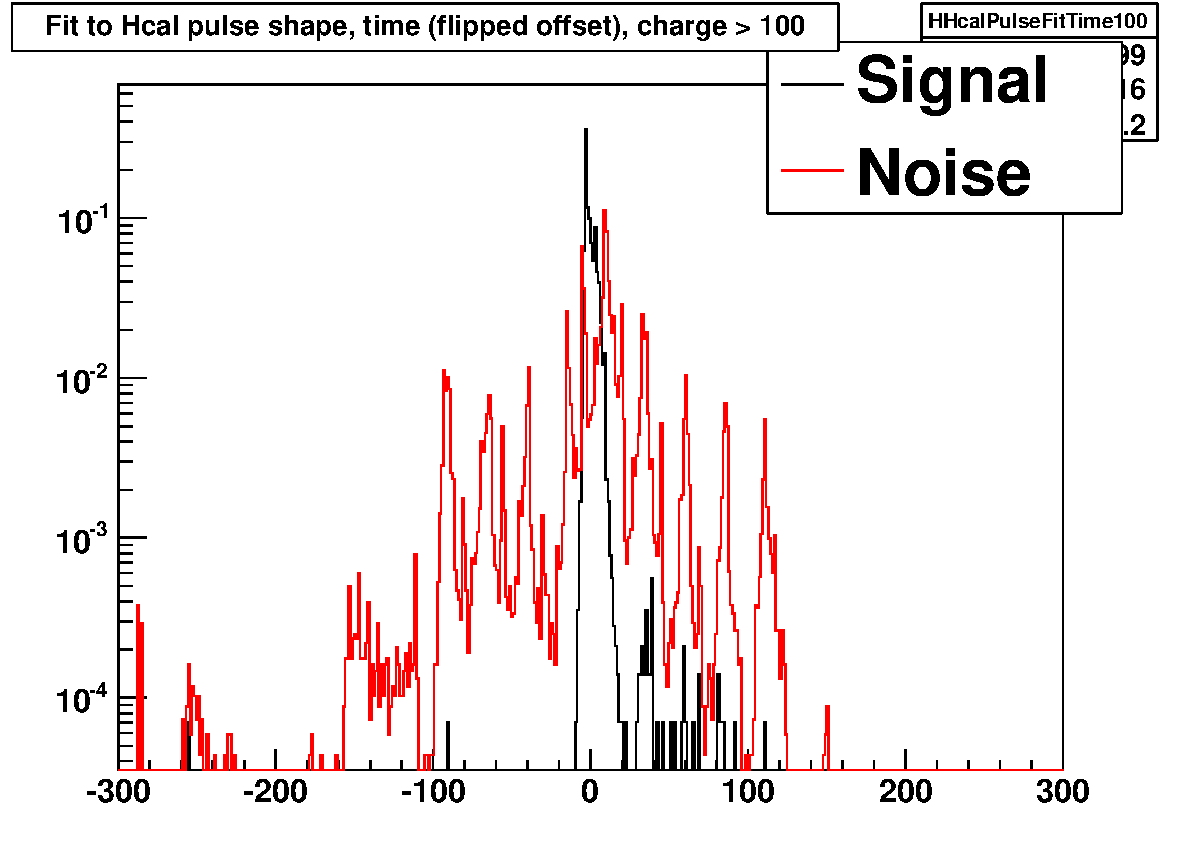
\includegraphics[width=120mm]{DailyLog/6275/6275HHcalPulseFitTime100.pdf}
\caption{Peak time from fit for pulse with charge at least 100 fC}
\label{Figure_6275HHcalPulseFitTime100}
\end{figure}

\begin{figure}
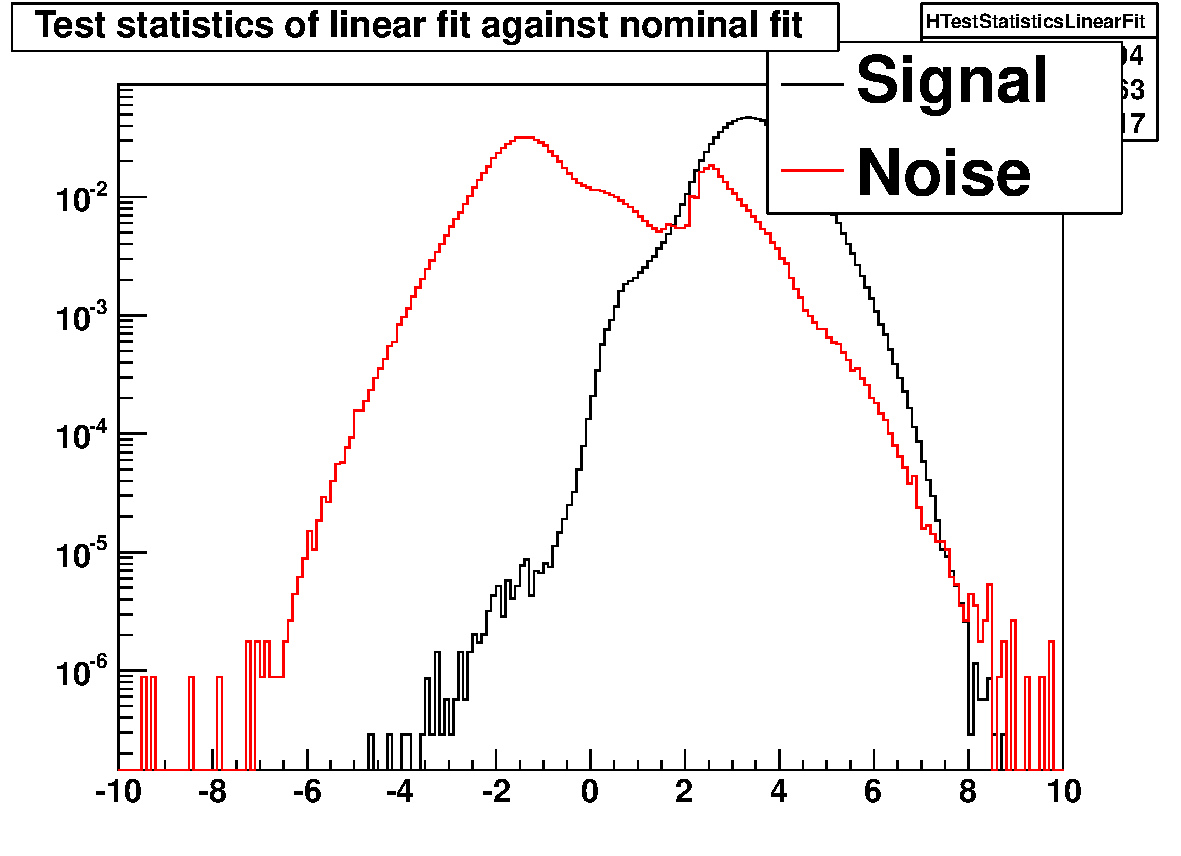
\includegraphics[width=120mm]{DailyLog/6275/6275HTestStatisticsLinearFit.pdf}
\caption{Test statistics on linear fit.}
\label{Figure_6275HTestStatisticsLinearFit}
\end{figure}

\begin{figure}
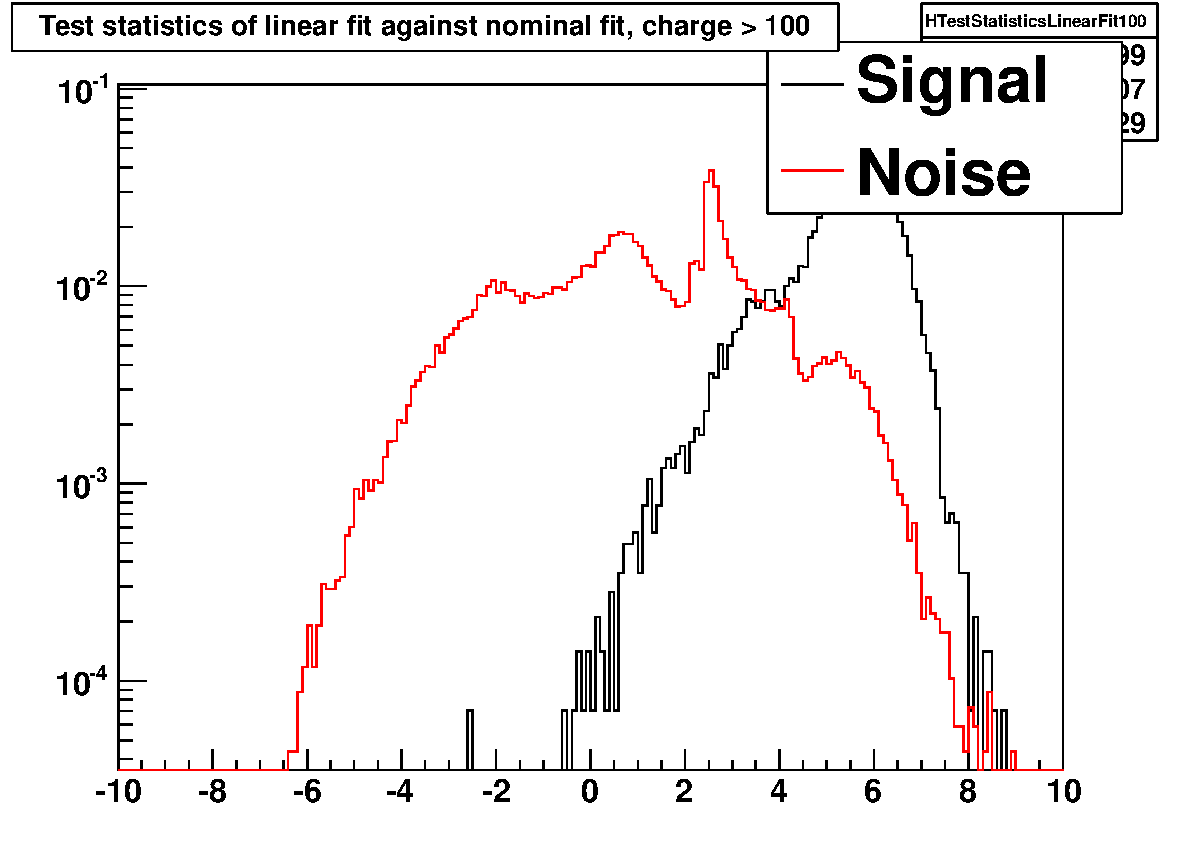
\includegraphics[width=120mm]{DailyLog/6275/6275HTestStatisticsLinearFit100.pdf}
\caption{Test statistics on linear fit, charge \textgreater 100 fC.}
\label{Figure_6275HTestStatisticsLinearFit100}
\end{figure}

\begin{figure}
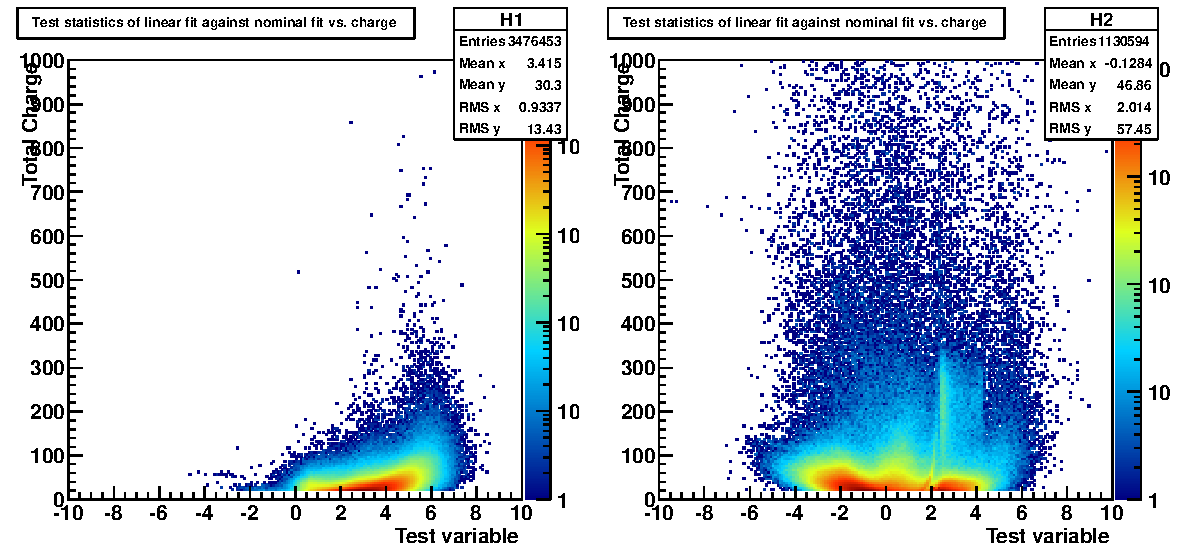
\includegraphics[width=120mm]{DailyLog/6275/6275HTestStatisticsLinearFitVsCharge.pdf}
\caption{Test statistics on linear fit.  Left: signal, right: noise}
\label{Figure_6275HTestStatisticsLinearFitVsCharge}
\end{figure}

\begin{figure}
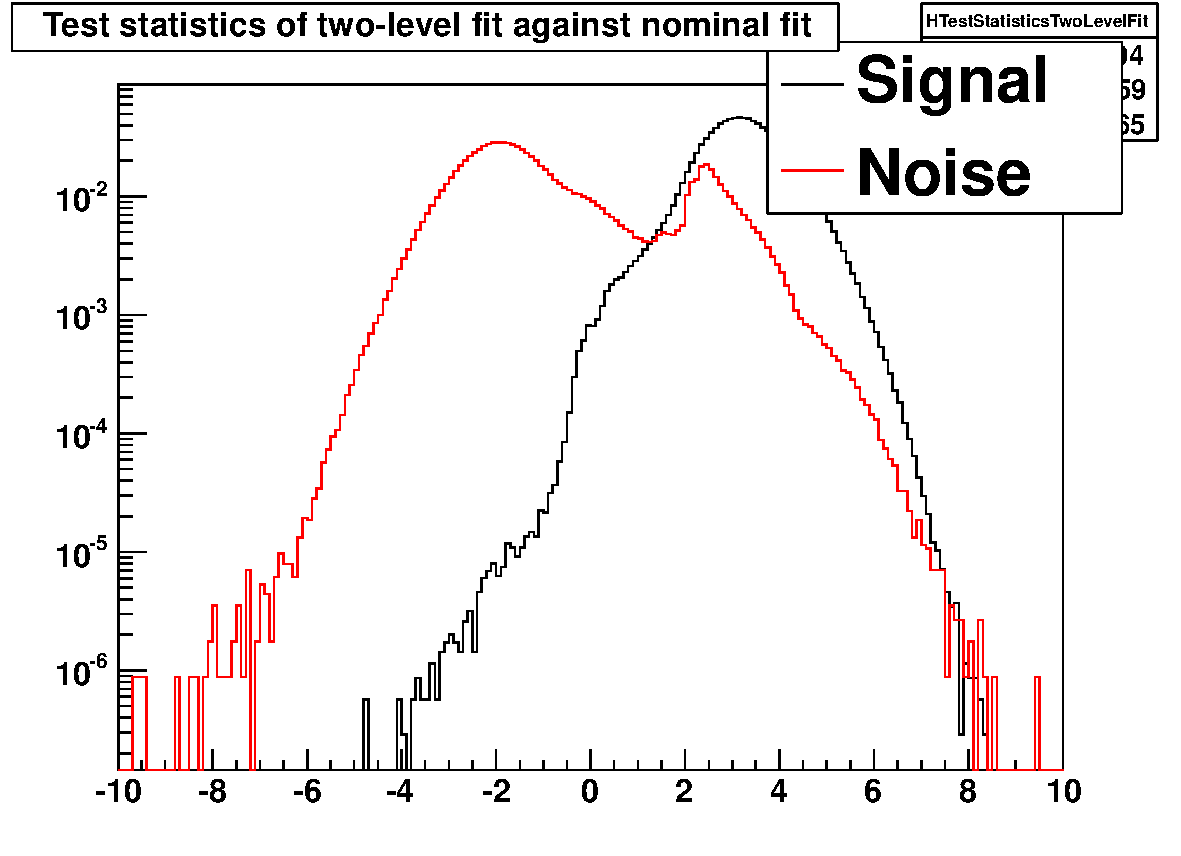
\includegraphics[width=120mm]{DailyLog/6275/6275HTestStatisticsTwoLevelFit.pdf}
\caption{Test statistics on two-level fit.}
\label{Figure_6275HTestStatisticsTwoLevelFit}
\end{figure}

\begin{figure}
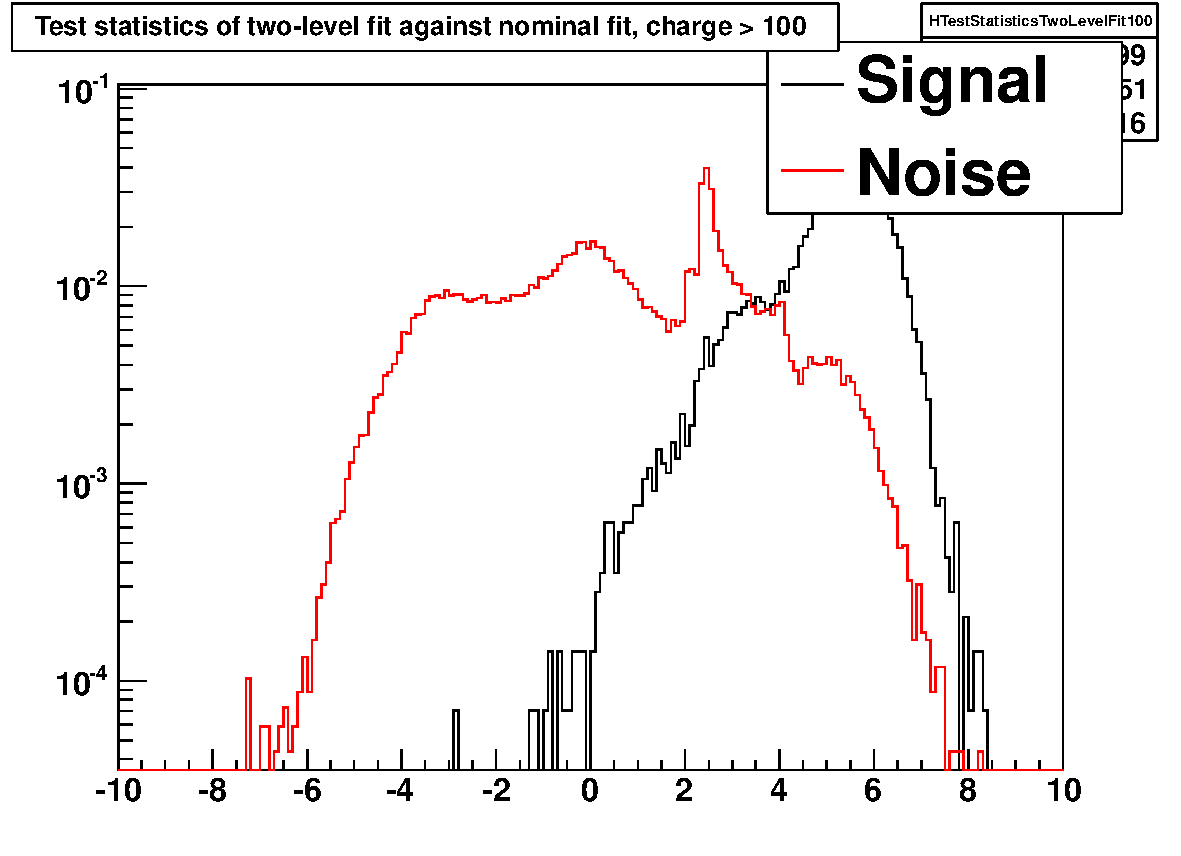
\includegraphics[width=120mm]{DailyLog/6275/6275HTestStatisticsTwoLevelFit100.pdf}
\caption{Test statistics on two-level fit, charge \textgreater 100 fC.}
\label{Figure_6275HTestStatisticsTwoLevelFit100}
\end{figure}

\begin{figure}
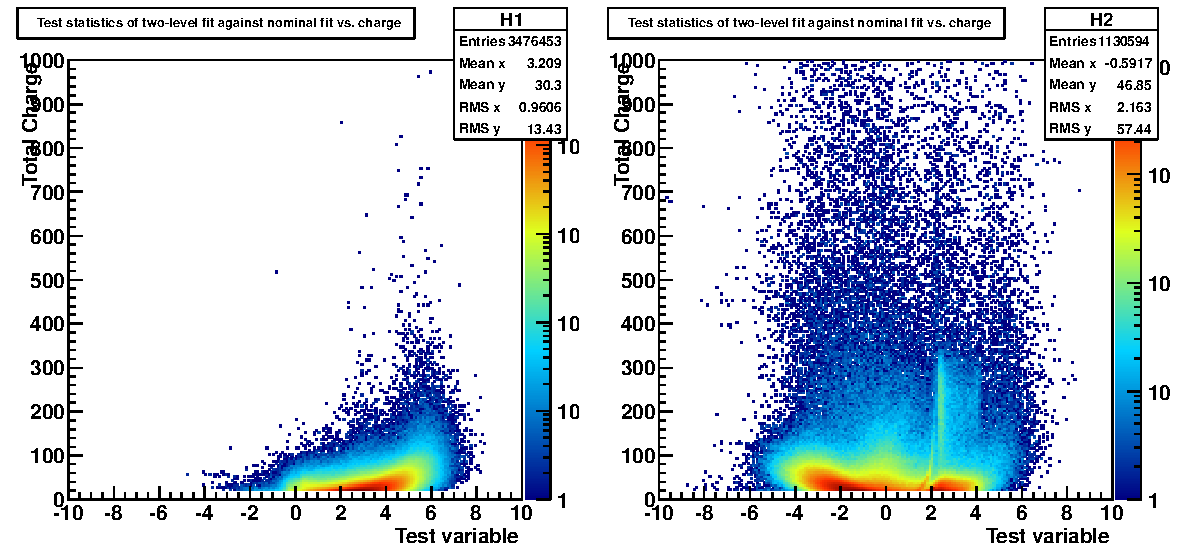
\includegraphics[width=120mm]{DailyLog/6275/6275HTestStatisticsTwoLevelFitVsCharge.pdf}
\caption{Test statistics on two-level fit.  Left: signal, right: noise}
\label{Figure_6275HTestStatisticsTwoLevelFitVsCharge}
\end{figure}

\begin{figure}
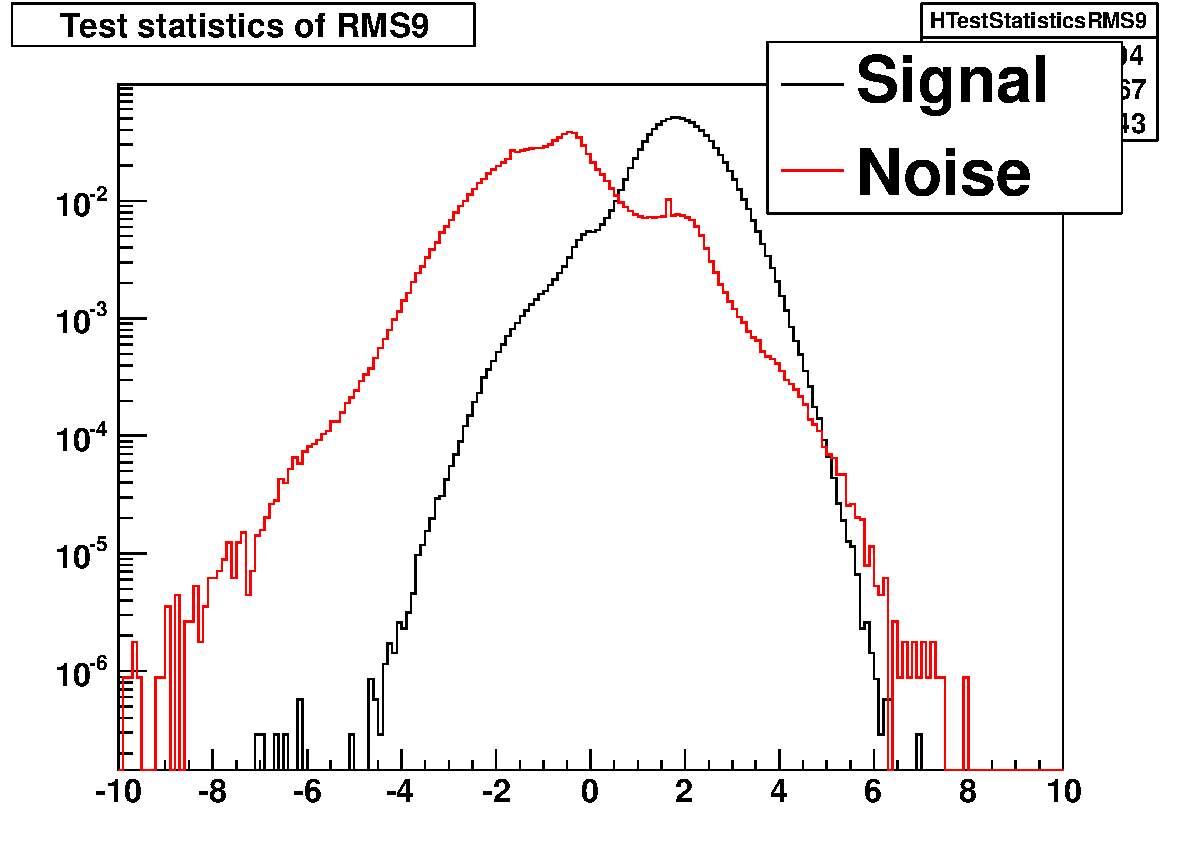
\includegraphics[width=120mm]{DailyLog/6275/6275HTestStatisticsRMS9.pdf}
\caption{Test statistics on RMS9.}
\label{Figure_6275HTestStatisticsRMS9}
\end{figure}

\begin{figure}
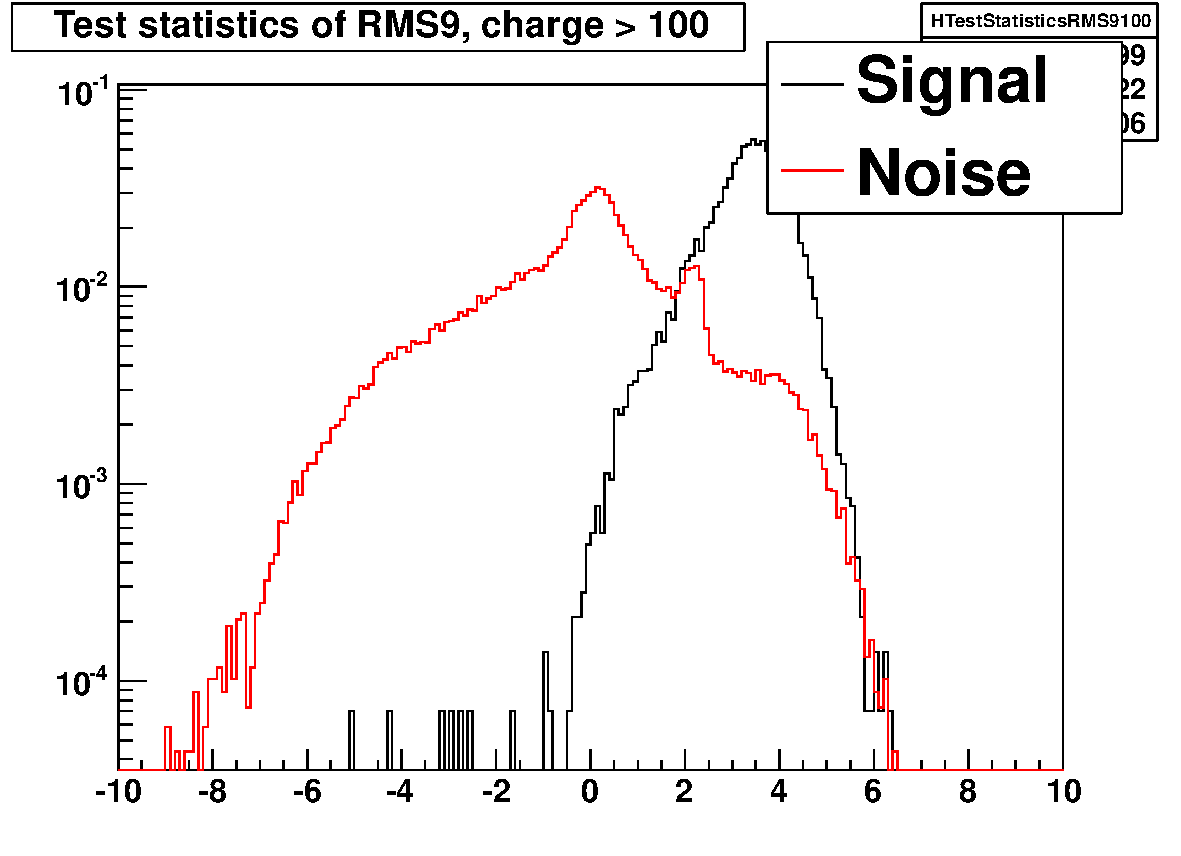
\includegraphics[width=120mm]{DailyLog/6275/6275HTestStatisticsRMS9100.pdf}
\caption{Test statistics on RMS9, charge \textgreater 100 fC.}
\label{Figure_6275HTestStatisticsRMS9100}
\end{figure}

\DailySection{Artur's request of vecbos ntuples}

\begin{enumerate}
\item \texttt{/JetMET/Run2010A-Sep17ReReco\_v2/RECO}         (Run Range 141956-144114)
\item \texttt{/Jet/Run2010B-PromptReco-v2/RECO}                   (Run Range 146240-147370)
\item \texttt{/METFwd/Run2010B-PromptReco-v2/RECO}          (Run Range 146240-147370)
\end{enumerate}

Will begin running during the weekend, and hopefully they will finish early next week.


\DailySection{Reflection}

\DailySection{Goals for next work day}

\begin{enumerate}
\item Eat lunch
\item Eat dinner
\item Find the red herring
\end{enumerate}


